%% FEL CVUT

\documentclass[journal]{IEEEtran}
\usepackage{graphicx}


\begin{document}
%
% paper title
\title{Multi-Agent Systems Using Kobuki Turtlebots:\\Leader-Follower Premise}
\author{Sinchiguano Cesar}


\markboth{Intelligent and Mobile Robotics Group, Czech Technical University in Prague, 20018/19}{Shell \MakeLowercase{\textit{et al.}}: Bare Demo of IEEEtran.cls for Journals}
\maketitle

%done
\begin{abstract}

%%%%%%%%%%%%%%%%%
Multi-agent system is a topic that has generated a lot interest in the research community. This interest is because a multi-agent systems present a more robust and cheaper solution to a certain tasks that are better performed using several low-cost robots rather than a single one. Multi-agent system can be achieved through many approaches. The approach used in this report is the one based on the leader-follower premise.
\end{abstract}


\section{Introduction}

%%%%%%%%%%%%%%%%%%%%%%%%%%%%%%%

Multi-robot systems present a more robust and cheaper solution to certain tasks that are better performed using several low-cost robots rather than a single one. This gives rise to the formation control problem. The formation problem has been regarded as an important problem in multi-robot systems where the goal is to make a fleet of autonomous mobile robots move toward and maintain a desired geometric shape. According to the survey presented in (Guanghua et al., 2013), and the references therein, formation structure can be divided into three strategies: the leader–follower strategy, the behavioural and the virtual structure approaches. Several approaches have been proposed in the literature to solve this problem. However, most of the existing literature tackle the theoretical side of the problem mainly the controller design. Nevertheless, some of them have carried on real experiments to prove the effectiveness of their proposed controller. 

In this report, we propose the use of ROS as a new framework so that real experiments for the formation control problem can be conducted effectively. Due to its simplicity and scalability, the leader-follower approach is considered in this paper also. However, the proposed framework can be extended so that other formation strategies or consensus algorithm can be implemented. 
The rest of this paper will be organized as follow: The introduction about ROS concepts is highlighted in Section II, with the software setup in Section III, followed by a detailed explanation of the software processes and the needed ROS packages are presented  in Section IV, finally conclusions drawn from this experiment and some future work directions in Section VI

%%%%%%%%%%%%%%%%%%%%%%
%%%%%%%%%%%%%%%%%%%%%%


\begin{enumerate}
\item \textbf{Log.....}

Gi \cite{temp1}........

\begin{figure}[!h]
\begin{center}
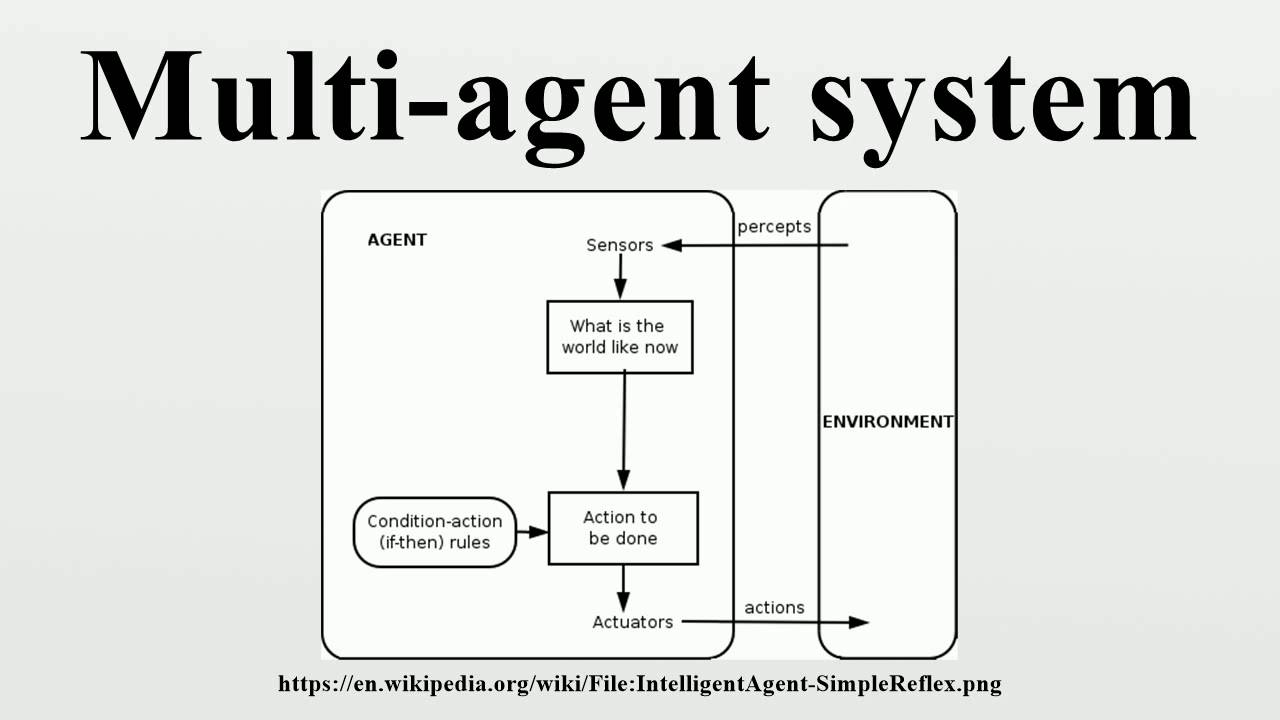
\includegraphics[width=2in]{one.jpg}
\caption{An example of multi-agent system. \cite{temp1}}
\end{center}
\label{fig:mypicture1}
\end{figure}


%%%%%%%%%%%%%%%%%%%%%%
%%%%%%%%%%%%%%%%%%%%%%
\item \textbf{AdaBoost classifier}

AdaBoost........:





%%%%%%%%%%%%%%%%%%%%%%
%%%%%%%%%%%%%%%%%%%%%%
\item \textbf{Random Forest classifier}

Th.......


%%%%%%%%%%%%%%%%%%%%%%
%%%%%%%%%%%%%%%%%%%%%%
\item \textbf{Naive Bayesian (NB) Classifier}


\end{enumerate}

%%%%%%%%%%%%%%%%%%%%%%%%%%%%%
%%%%%%%%%%%%%%%%%%%%%%%%%%%%%%%


\section{Backgroung}
%done
\begin{enumerate}
\item \textbf{Robotic Operating System (ROS)}\\
ROS is a flexible framework for writing robot software. It is a collection of tools, libraries, and conventions that aim to simplify the task of creating complex and robust robot behaviour across a wide variety of robotic platforms . It is based on the concepts of nodes, topics, messages and services. A node is an executable program that performs computation. Nodes need to communicate with each other to complete the whole task. The communicated data are called messages. ROS provides an easy way for passing messages and establishing communication links between nodes, which are running independently. They pass these messages to each other over a Topic, which is a simple string. However, topics are asynchronous, synchronous communication is provided by services. Services act in a call-response manner where one node requests that another node execute a one-time computation and provide a response. For more details about ROS, the reader can refer to \cite{temp2}.



\item \textbf{Architecture of the System}

T.........

\end{enumerate}


%%%%%%%%%%%%%%%%%%%%%%%
%%%%%%%%%%%%%%%%%%%%%%%
%working on
\section{Experimental setup}

The test space consist of two Kobuki TurtleBots. It is a low-cost, open source differential drive robot. It consists of a mobile base, an RGB-D sensor and an CPU making it a perfect entry-level mobile robot platform. The Kobuki was chosen because it is an open source UGV (Unmanned ground vehicle) platform, making it perfect for research and development. The Kobuki SDK (Software development kit) is based on ROS, which is the preferred development platform by the Intelligent and Mobile Robotics Group because of its intuitive publisher/subscriber message passing structure that allows robust and simple communication within multiple facets of a robotic system.

\begin{figure}[!h]
\begin{center}
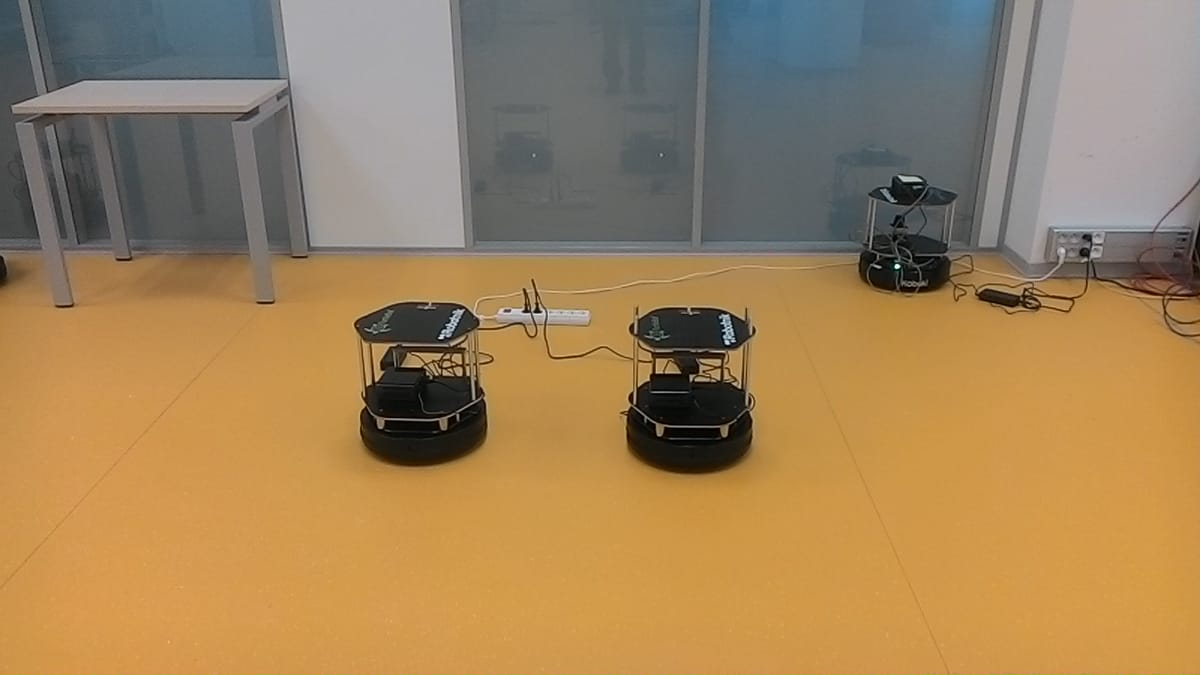
\includegraphics[width=2in]{two.jpg}
\caption{Two turtlebots used in the experimental test bed.}
\end{center}
\label{fig2:mypicture2}
\end{figure}


The Fig 2 shows two Turtlebots which are equipped with a Kinect Sensor. The robots run ROS (Robot Operating System), and are supported by various ROS libraries. 

\ref{fig2:mypicture2}

C.......

%in process
\begin{enumerate}

\item Logistic Regression classifier


%%%%%%%%%%%%%%%%%%%%%%%%%%%%%
%%%%%%%%%%%%%%%%%%%%%%%%%%%%%
%%%%%%%%%%%%%%%%%%
%%%%%%%%%%%%%%%%%%
\item Naive Bayesian Classifier\\
Wication.

\begin{enumerate}
\item Grid Search\\
W....er and $ngram_{\_}range$ as a pahe $ngram_{\_}range$ dand $bi-grams$ in t...ns.
 




\item Best parameters


\end{enumerate}
\end{enumerate}





%%%%%%%%%%%%%%%%%%%%%%%%%%%%%%%%%%%%%%%%%%%%%%%%%%%%%%%%%%%%%%%%%%%%%%%%%

\section{Software Processes}

Af.......

\begin{enumerate}
\item \textbf {Simulating Multiple Turtlebots in Gazebo}\\
This is an example of simulating and controlling multiple Turtlebot robots. It is built as an extension of the Simulating Turtlebot tutorial on \cite{temp4}.

\begin{figure}[!h]
\begin{center}
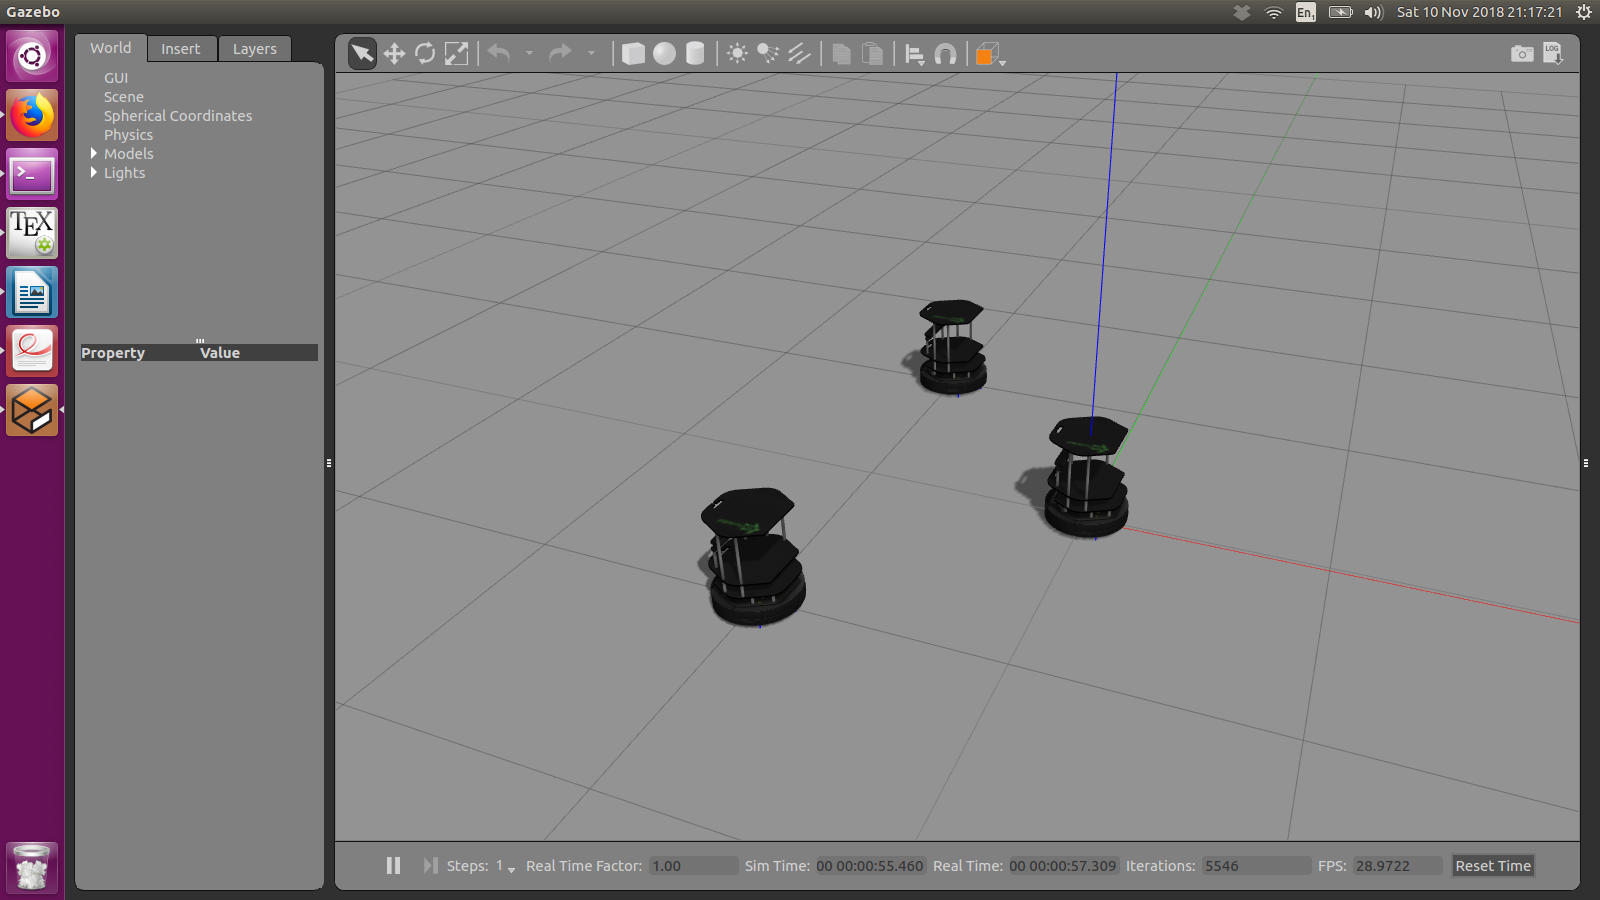
\includegraphics[width=2in]{two.png}
\caption{A general view of the system.}
\end{center}
\label{fig:mypicture3}
\end{figure}

\begin{enumerate}
\item \textbf {Quick Start}

The main.launch file is a working example that instantiates two simulated Turtlebots in Gazebo. 

You will first need to install the following packages in your workstation:
\begin{enumerate}
\item {turtlebot}\cite{temp6}.
\item {kobuki}\cite{temp8}.
\item {turtlebot{\_}simulator}\cite{temp7}.
\item {turtlebot{\_}interactions}\cite{temp9}.
\end{enumerate}
Then after you have these packages in your workspace, place the multi{\_}agents\cite{temp5} package in your src diretory.\\
As long as all of the system dependencies of your packages are installed, we can now build your new packages.\\
In a catkin workspace

\begin{enumerate}
\item {{\$} catkin{\_}make}.
\end{enumerate}

Before continuing source your new setup.*sh file:
\begin{enumerate}
\item {{\$} source devel/setup.bash}.
\end{enumerate}

To make sure your workspace is properly overlayed by the setup script, make sure ROS{\_}PACKAGE{\_}PATH environment variable includes the directory you are in with the following command:

{\$} echo {\$}ROS{\_}PACKAGE{\_}PATH



%%%%%%%%%%%%%%%%%%%%%%%%%%%%%%%%%%%%%%%%%%%%%%%
\item \textbf {Description: multi{\_}agents package}


If everything was done with the commands above then it should just work. From there, to learn what it does, I woud recommend going over the multi{\_}agent.launch, one{\_}turle.launch and main.launch files those who can be located inside your catkin{\_}ws with the following command:\\
{\$} cd src/multi{\_}agents/launch \\
which will lead you to the launch files mentioned above. All of them are binding one another. The only one that it should be launched is the one named as main.launch file which does the heavy lifting of setting up each Turtlebot. Here is a high-level outline of what this package does.

main2.launch:
\begin{enumerate}
\item {Starts Gazebo (both the sim engine and the gui)}
\item {Start some visualization and debugging tools (rviz,rqt{\_}console, etc.)}
\item {For each instance of a Turtlebot, setup the namespace, and define the initial}
\item {multi{\_}agents.launch}

\begin{enumerate}
\item {Accept namespace and initial pose arguments from multihusky.launch}.
\item {Set the tf{\_}prefix based on the namespace}
\item {Call a xacro robot{\_}description with namespace and tf{\_}prefix arguments}
\item {Spawn the Turtlebot model in Gazebo using gazebo{\_}ros}
\item {Start a robot{\_}state{\_}publiser node}
\item {Start a static{\_}transform{\_}publisher node to establish the tf transfrom from the map to the specific odom frame.}
\end{enumerate}
\end{enumerate}
Here are some screen captures and images to illustrate what you should see if things are working properly.
    
 

Four Turtlebot robots in Gazebo




\begin{figure}[!h]
\begin{center}
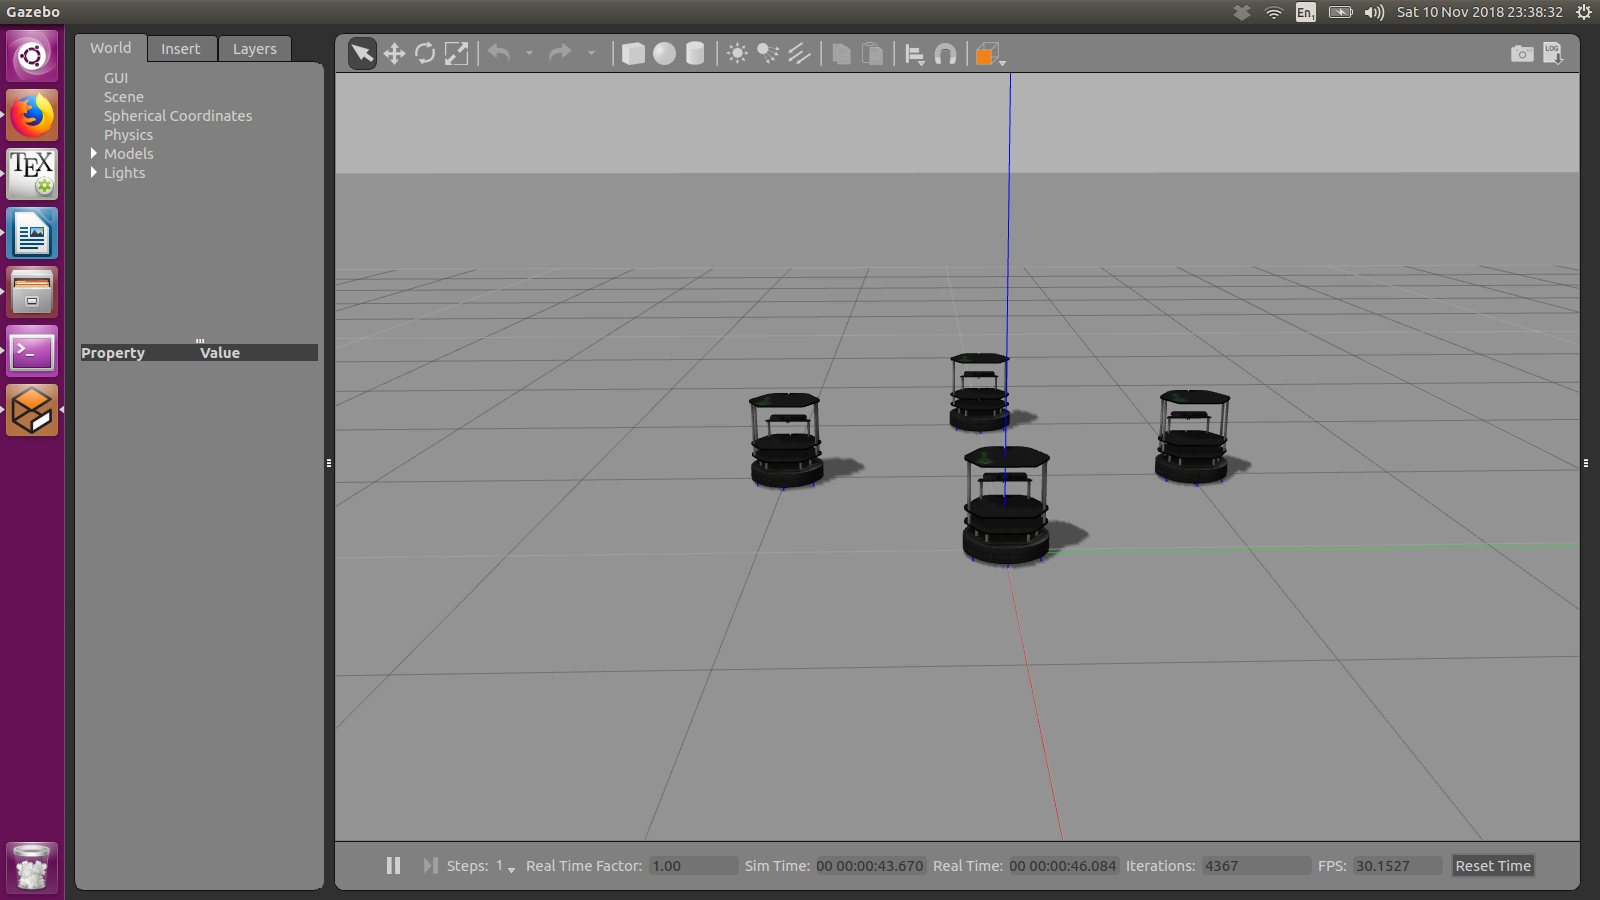
\includegraphics[width=2in]{three.png}
\caption{A general view of the system with four multi-agents.}
\end{center}
\label{fig:mypicture4}
\end{figure}





\end{enumerate}

\end{enumerate}






\section{Conclusion}
j.....


%%%%%%%%%%%%%%%%
%%%%%%%%%%%%%%%%%%
%%%%%%%%%%%%%%%%%%%%

\begin{thebibliography}{1}

\bibitem{temp1}
\bibitem{temp2}
\bibitem{temp3}
http://www.ros.org/about-ros/
\bibitem{temp4}
http://wiki.ros.org/turtlebot/Tutorials/indigo
\bibitem{temp5}
https://github.com/Sinchiguano/Multi-agent-system/tree/master/src/multi{\_}agents
\bibitem{temp6}
http://wiki.ros.org/turtlebot
\bibitem{temp7}
http://wiki.ros.org/turtlebot{\_}simulator
\bibitem{temp8}
http://wiki.ros.org/kobuki
\bibitem{temp9}
http://wiki.ros.org/turtlebot{\_}interactions

\bibitem{temp10}
\bibitem{temp11}

\end{thebibliography}

\end{document}





%
%

I implemented in the supplied filter.py module as the function called $modified_{\_}accuracy$ which uses the confusion matrix feature to compute TP, FP, TN, FN.

$$macc=\frac{n_{TP}+n_{TN}}{n_{TP}+n_{TN}+10*n_{FP}+n_{FN}}$$